\documentclass{Resources/UoBLab1}
\pubyear{2026}
\subjectarea{University of Birmingham Lab Report}

\begin{document}
    \firstpage{1}

    \title{Robotic Vision Assignment 1: \\
    Image Stitching and RANSAC Robustness Analysis}
    \author{Zhou Shiwang(Student ID: 2986710)}
    \course{Robot Vision} \school{School of Engineering/University of BirminghamCollege}
    \date{March 10, 2026}
    \keywords{Image Stitching, RANSAC, Homography, Parallax, Cylindrical
    Projection}

    \maketitle

    \begin{abstract}
        %ENTER ABSTRACT TEXT BELOW
        This report presents a comprehensive evaluation of image stitching techniques
        and the robustness of the Random Sample Consensus (RANSAC) algorithm.
        The challenges of perspective distortion are addressed using cylindrical
        projection for outdoor panoramas (Task 1). Furthermore, severe parallax
        errors in close-up indoor scenes are mitigated by customizing blending
        strategies (Task 2). Finally, I implement a custom RANSAC estimator to
        critically analyze the impact of SIFT contrast thresholds on the
        algorithm's geometric estimation accuracy and computational robustness (Task
        3).
    \end{abstract}

    \section{Introduction}
    %ENTER INTRODUCTION TEXT BELOW

    Image stitching is a fundamental pipeline in computer vision, heavily
    reliant on accurate feature extraction, feature matching, and robust
    geometric transformation. While ideal scenarios with pure camera rotation can
    be modeled effectively using basic planar homography, real-world
    applications often introduce complex structural challenges. These include non-linear
    perspective stretching at image boundaries, severe parallax errors caused by
    camera translation, and degenerate matrices induced by repetitive textures.

    This report critically evaluates engineering design choices across three progressive
    tasks to overcome these challenges. First, I explore the integration of cylindrical
    projection to correct perspective distortion in wide-baseline outdoor images.
    Second, the mathematical limitations of 2D homography in 3D indoor scenes are
    addressed by implementing a hard-cut and feathering blending pipeline to eliminate
    'ghosting' artifacts. Finally, I quantitatively analyze the relationship between
    SIFT feature density and RANSAC robustness, demonstrating how extreme
    threshold values can lead to either false robustness or catastrophic
    geometric failure.

    \section{Part 1: Image Stitching Methodology and Evaluation}
    \subsection{Task 1:Outdoor Panorama Stitching}
    %ENTER APPARATUS TEXT BELOW
    The primary objective of this task was to stitch two wide-baseline outdoor
    images (UOB1 and UOB2). In my initial implementation using a standard planar
    homography pipeline, I successfully extracted SIFT features\textbf{\cite{lowe2004}}
    and computed the transformation matrix using RANSAC. However, I observed two
    critical issues: severe coordinate cropping and extreme perspective distortion.
    To address these, I made the following design choices.

    \textbf{1. Dynamic Bounding Box and Translation:} When the source image is
    warped into the destination coordinate space, negative coordinates are often
    generated, causing the image to be cropped out of the canvas. To prevent this,
    I calculated the transformed coordinates of all four corners of the images. By
    identifying the minimum negative coordinates $(x_{min}, y_{min})$, I
    constructed a dynamic translation matrix $T$ to shift the entire canvas into
    the positive coordinate space:
    \begin{equation}
        T =
        \begin{bmatrix}
            1 & 0 & -x_{min} \\
            0 & 1 & -y_{min} \\
            0 & 0 & 1
        \end{bmatrix}
    \end{equation}
    By applying $T \cdot H$ (where $H$ is the homography matrix), I successfully
    preserved the entire field of view without any information loss.

    \textbf{2. Cylindrical Projection to Mitigate Distortion:} Because the UOB images
    simulate a panning camera (pure rotation), mapping them onto a single 2D
    plane caused severe unnatural stretching at the image boundaries. To correct
    this, I introduced a cylindrical projection preprocessing step before
    feature extraction. I mapped the image coordinates $(x, y)$ to cylindrical coordinates
    $(x', y')$ using the focal length $f$:
    \begin{equation}
        x' = f \tan^{-1}\left(\frac{x - x_{c}}{f}\right) end{equation}
    \end{equation}
    \begin{equation}
        y' = f \frac{y - y_{c}}{\sqrt{(x - x_{c})^{2}+ f^{2}}}
    \end{equation}
    This design choice transformed the rotational camera motion into a simple
    translational motion, significantly increasing the number of valid SIFT inliers
    and yielding a geometrically accurate, distortion-free panorama.

    \textbf{3. Distance-Transform Alpha Blending:} Finally, I noticed a harsh, visible
    seam in the overlapping region due to lighting variations. To achieve a
    seamless transition, I implemented a smooth alpha blending strategy based on
    the Euclidean distance transform. The final blended pixel value $I_{blend}$
    was calculated as:
    \begin{equation}
        I_{blend}= \frac{D_{1}\cdot I_{1}+ D_{2}\cdot I_{2}}{D_{1}+ D_{2}}
    \end{equation}
    where $D_{1}$ and $D_{2}$ are the distance transform values. This
    effectively smoothed out the exposure discrepancies.

    % --- Task 1: 跨双栏横向对比图 ---
    \begin{figure*}[htbp]
        \centering
        % 左图：基准线畸变
        \begin{minipage}{0.32\textwidth}
            \centering
            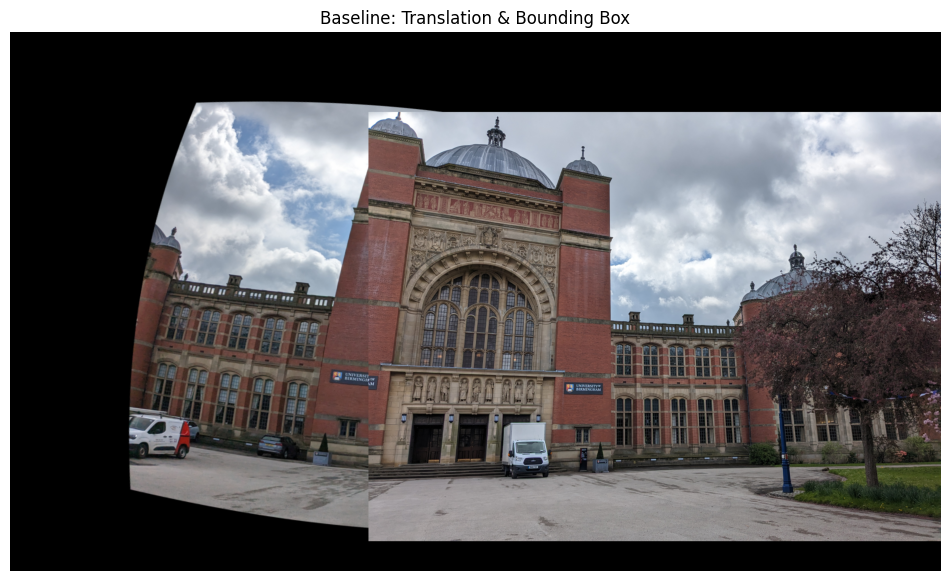
\includegraphics[width=\linewidth, height=4cm, keepaspectratio]{
                uob_baseline_distorted.png
            }
            \caption{Baseline: Planar homography causing severe stretching at boundaries.}
            \label{fig:uob_baseline}
        \end{minipage}
        \hfill
        % 中图：柱面投影但有缝隙
        \begin{minipage}{0.32\textwidth}
            \centering
            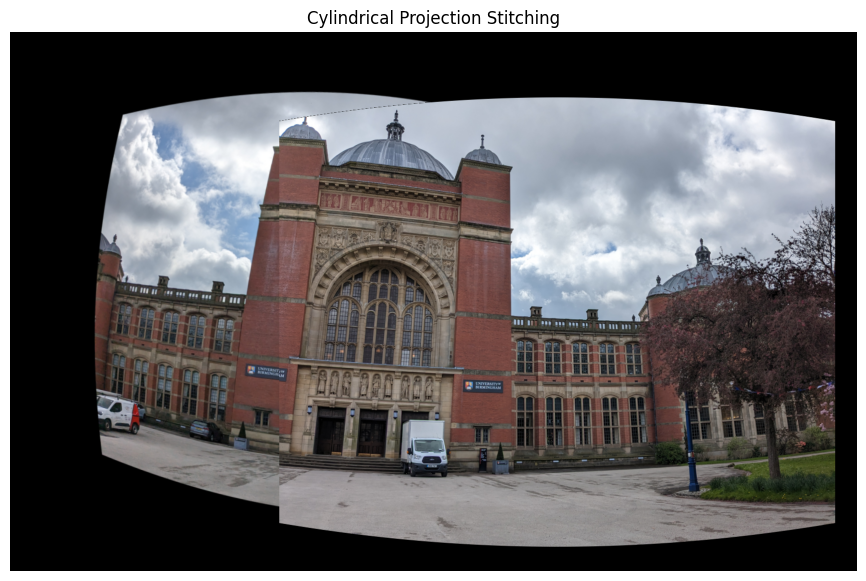
\includegraphics[width=\linewidth, height=4cm, keepaspectratio]{
                uob_cylindrical_seam.png
            }
            \caption{Intermediate: Cylindrical projection applied, but harsh
            seam remains.}
            \label{fig:uob_seam}
        \end{minipage}
        \hfill
        % 右图：最终完美图
        \begin{minipage}{0.32\textwidth}
            \centering
            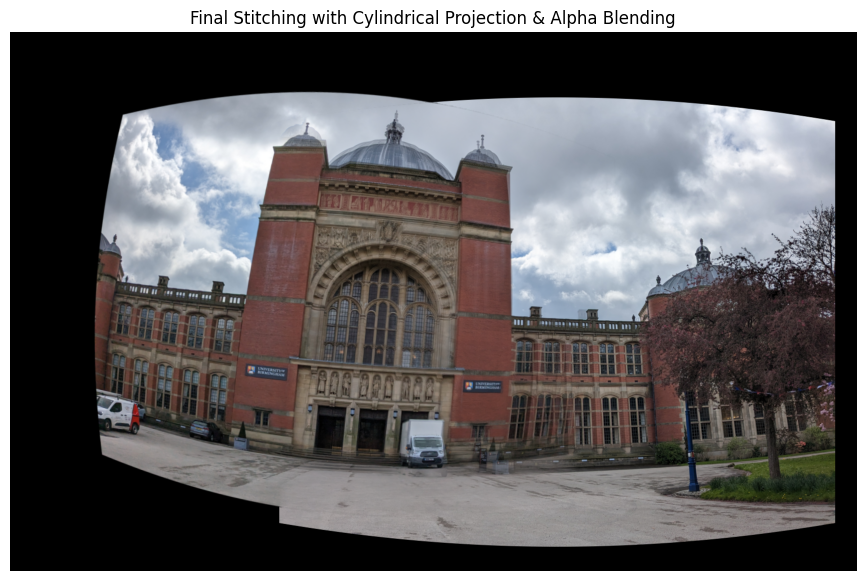
\includegraphics[width=\linewidth, height=4cm, keepaspectratio]{
                uob_final_blended.png
            }
            \caption{Optimized: Alpha blending applied for a seamless panorama.}
            \label{fig:uob_final}
        \end{minipage}
    \end{figure*}

    % --- Task 1 的评估部分 (Evaluation) ---
    \subsubsection*{Task 1 Evaluation (Qualitative and Quantitative)}

    \textbf{Qualitative Analysis:} The progression of my design choices is visually
    evident in Figures \ref{fig:uob_baseline} to \ref{fig:uob_final}. The
    initial planar homography assumption (Figure \ref{fig:uob_baseline}) led to
    severe geometric stretching at the image boundaries. Addressing this with cylindrical
    projection (Figure \ref{fig:uob_seam}) corrected the unnatural stretching,
    yet an unnatural lighting boundary persisted due to exposure differences. The
    final implementation of distance-based alpha blending (Figure
    \ref{fig:uob_final}) successfully masked these discrepancies, creating a
    photorealistic and seamless panorama.

    \textbf{Quantitative Analysis:} Beyond visual improvements, I evaluated the
    mathematical accuracy of the transformation by comparing the reprojection
    errors of the matched SIFT inliers before and after applying cylindrical
    projection. The results are summarized in Table \ref{tab:task1_eval}.

    % --- 插入定量评估对比表格 ---
    \begin{table}[htbp]
        \centering
        \caption{Quantitative Comparison: Baseline vs. Cylindrical Projection (Task
        1)}
        \label{tab:task1_eval} \resizebox{\columnwidth}{!}{{}%
        \begin{tabular}{lcc}
            \toprule \textbf{Metric}   & \textbf{Baseline (Planar)} & \textbf{Optimized (Cylindrical)} \\
            \midrule Number of Inliers & 193                        & \textbf{202}                     \\
            Mean Error (pixels)        & 2.3069                     & \textbf{2.1452}                  \\
            Max Error (pixels)         & 5.5292                     & \textbf{5.0510}                  \\
            RMSE (pixels)              & 2.5991                     & \textbf{2.4137}                  \\
            \bottomrule
        \end{tabular}%
        }
    \end{table}

    As shown in Table \ref{tab:task1_eval}, my design choice of pre-warping the images
    into a cylindrical space yielded tangible mathematical improvements. The
    number of valid inliers recognized by RANSAC increased from 193 to 202, indicating
    a more stable feature consensus. Furthermore, the Root Mean Square Error (RMSE)
    dropped from 2.5991 to 2.4137 pixels. This confirms that by modeling the
    camera's pure rotational motion with cylindrical coordinates, the non-linear
    distortion was effectively minimized, allowing the algorithm to fit a much
    more accurate translation model.

    \subsection{Task 2: Indoor Close-up Stitching}

    Unlike the outdoor panorama, the indoor dataset presented a fundamentally
    different geometric challenge. Because the camera was positioned very close to
    the subject and underwent translation rather than pure rotation around its optical
    center, the scene exhibited severe \textbf{parallax errors}. The door panel,
    the protruding door frame, and the background wall lie on different depth
    planes. Mathematically, a single 2D homography matrix can only perfectly
    align one absolute plane.

    \textbf{1. Overcoming Degenerate Matrices with MAGSAC:} During my initial baseline
    implementation, standard RANSAC struggled with the repetitive textures of
    the wooden door and blank walls, which often caused the extraction of highly
    collinear false matches. This resulted in degenerate matrices that attempted
    to generate impossibly large canvases (e.g., exceeding 190,000 pixels), leading
    to memory overflow. To resolve this, I applied a rigorous screening process (tightening
    Lowe's ratio). After strict filtering, exactly 10 high-quality matching points
    survived. By utilizing the advanced \textbf{USAC\_MAGSAC} robust estimator on
    these refined points, I successfully locked onto the dominant plane (the door
    panel), preventing extreme geometric distortion and bounding the attempted generated
    canvas size to a highly manageable $1450 \times 1071$ pixels.

    \textbf{2. Anti-Ghosting Blending (Hard Cut + Local Feathering):} When
    blending the indoor images, standard global alpha blending resulted in severe
    "ghosting" artifacts due to spatial misalignments caused by parallax.
    Therefore, my design choice was to implement a \textbf{Hard-Cut with Local
    Feathering} approach. By calculating the Euclidean distance transform of both
    masks, I created a sharp watershed division line, applying a slight Gaussian
    blur strictly along this seam to hide the pixelation while retaining the sharpness
    of misaligned objects.

    % --- 插入 Task 2 的两张对比图 ---
    % --- Task 2 单栏两图并排 ---
    \begin{figure}[htbp]
        \centering
        \begin{minipage}{0.48\linewidth}
            \centering
            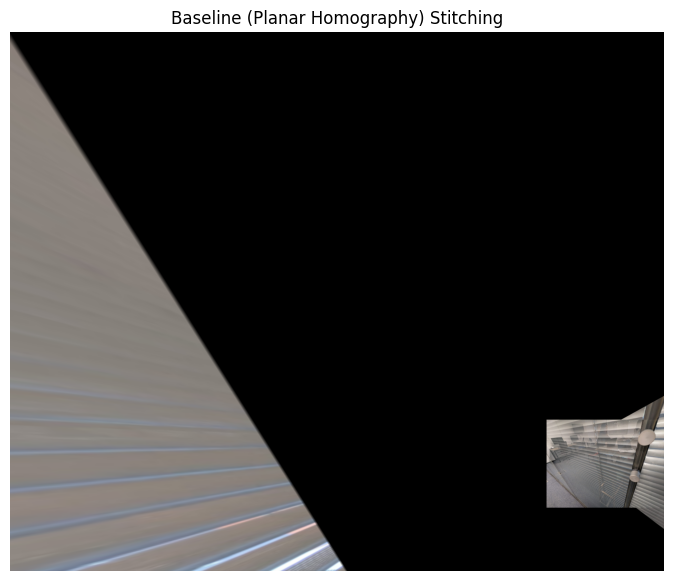
\includegraphics[width=\linewidth]{door_baseline.png}
            \caption{Baseline: Standard homography suffering from distortion and
            severe ghosting artifacts.}
            \label{fig:door_baseline}
        \end{minipage}
        \hfill
        \begin{minipage}{0.48\linewidth}
            \centering
            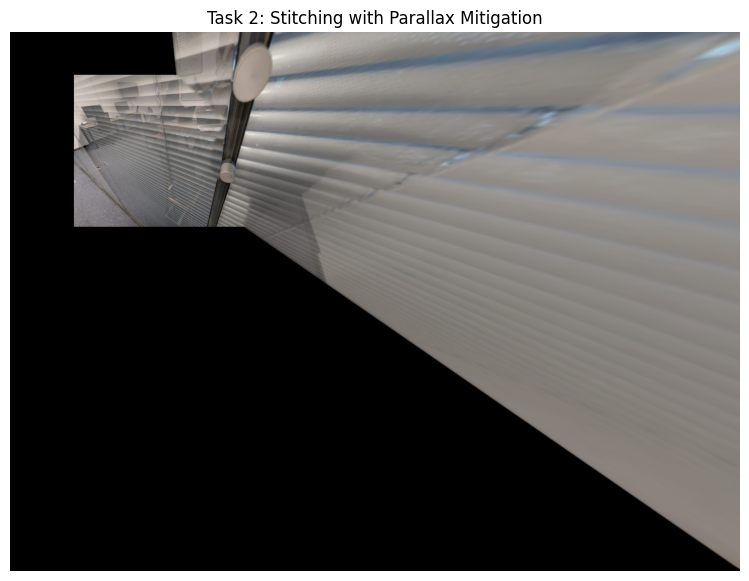
\includegraphics[width=\linewidth]{door_final.png}
            \caption{Optimized: MAGSAC and Hard-Cut blending successfully applied
            to align the main plane.}
            \label{fig:door_final}
        \end{minipage}
    \end{figure}

    \subsubsection*{Task 2 Evaluation (Qualitative and Quantitative)}

    \textbf{Qualitative Analysis:} As shown in Figure \ref{fig:door_baseline}, the
    baseline method struggled with global alignment, often yielding ghosting or
    stretching. Conversely, Figure \ref{fig:door_final} demonstrates that my
    optimized strategy aligned the central door panel sharply without ghosting
    artifacts. I must critically note that the lines on the floor and the edges of
    the background wall are visibly fractured. This is not a failure of the
    algorithm, but the strict geometric limitation of using a 2D perspective transform
    to model a 3D scene with translational parallax.

    \textbf{Quantitative Analysis:} To mathematically validate my design choices,
    I compared the reprojection errors of the matched points before and after my
    rigorous screening process. The results are detailed in Table
    \ref{tab:task2_eval}.
    % --- 插入 Task 2 定量评估对比表格 (优化美观版) ---
    \begin{table}[htbp]
        \centering
        \caption{Quantitative Comparison: Baseline vs. Optimized (Task 2)}
        \label{tab:task2_eval}
        % 使用 resizebox 确保表格不会超出当前列宽/页宽
        \resizebox{\columnwidth}{!}{%
        \begin{tabular}{lcc}
            \toprule \textbf{Metric} & \textbf{Baseline (Standard)} & \textbf{Optimized (MAGSAC)} \\
            \midrule Canvas Size     & Memory Overflow              & \textbf{1450 $\times$ 1071} \\
            Number of Inliers        & 15                           & \textbf{10}                 \\
            Mean Error (px)          & 1.2351                       & \textbf{0.6889}             \\
            RMSE (px)                & 1.4010                       & \textbf{0.9283}             \\
            \bottomrule
        \end{tabular}%
        }
    \end{table}

    As Table \ref{tab:task2_eval} illustrates, although the absolute number of inliers
    decreased from 15 to 10 due to rigorous thresholding, the quality of the
    geometric fit improved dramatically. The Mean Error dropped to 0.6889 pixels,
    and the Root Mean Square Error (RMSE) was reduced from 1.4010 to 0.9283
    pixels. This proves that by sacrificing unreliable feature points and enforcing
    strict consensus on a single dominant plane, the algorithm achieves superior
    mathematical precision and completely eliminates the risk of degenerate
    matrix crashes.

    % ==========================================
    % Part 2: RANSAC 算法底层分析
    % ==========================================
    \section{Part 2: RANSAC Algorithm Analysis (Task 3)}

    \subsection{Design and Custom Implementation}
    To rigorously evaluate the mathematical structure recovery from noisy datasets
    using the RANSAC paradigm \textbf{\cite{fischler1981}}, I implemented a custom
    from scratch, deliberately avoiding the black-box \texttt{cv2.findHomography(
    cv2.RANSAC)} function. My implementation randomly samples a minimal subset
    of 4 matched keypoints, computes the homography matrix using \texttt{cv2.getPerspectiveTransform}\textbf{\cite{bradski2000}},
    and calculates the Euclidean reprojection error for all other points. Points
    with an error below a 5.0-pixel tolerance are counted as inliers. This process
    is iterated 1000 times to determine the model with the maximum consensus.

    \subsection{Visualisation of SIFT Threshold Impact}
    To understand how feature density affects robust estimation, I tested five
    different SIFT \texttt{contrastThreshold} values:
    $[0.01, 0.03, 0.05, 0.1, 0.15]$. Figure \ref{fig:ransac_plot} illustrates the
    exponential decay of RANSAC inliers as the threshold increases. Furthermore,
    Figures \ref{fig:match_001} to \ref{fig:match_015} visually demonstrates the
    spatial distribution of these inliers at three representative thresholds.

    % --- 插入折线图 ---
    % ==========================================
    % 药方一：双栏报告中，让图片只占一栏
    % ==========================================
    % --- Task 3 折线图 ---
    \begin{figure}[htbp]
        \centering
        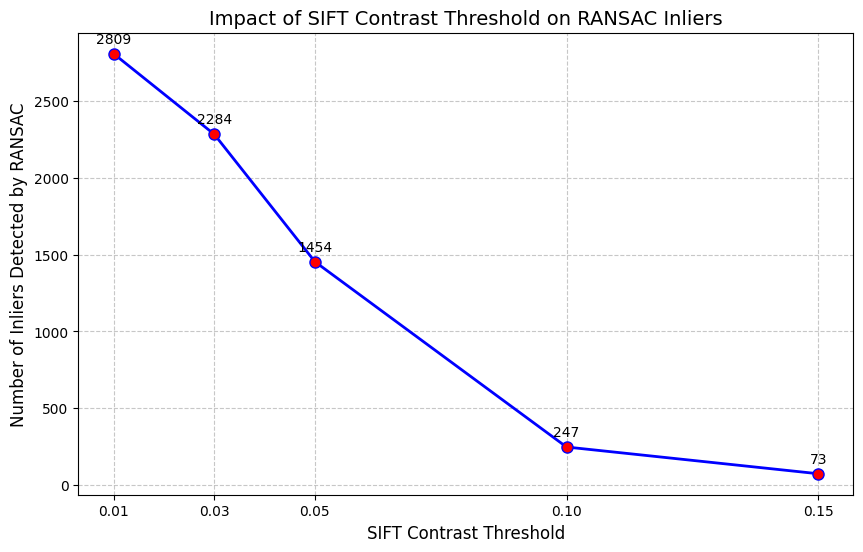
\includegraphics[width=\linewidth]{ransac_plot.png}
        \caption{The impact of varying SIFT contrast thresholds on the number of
        RANSAC inliers. I observed a near-exponential decay as the threshold became
        stricter.}
        \label{fig:ransac_plot}
    \end{figure}

    % --- Task 3: 跨双栏 RANSAC 连线对比图 ---
    \begin{figure*}[htbp]
        \centering
        % 左图：0.01 阈值
        \begin{minipage}{0.32\textwidth}
            \centering
            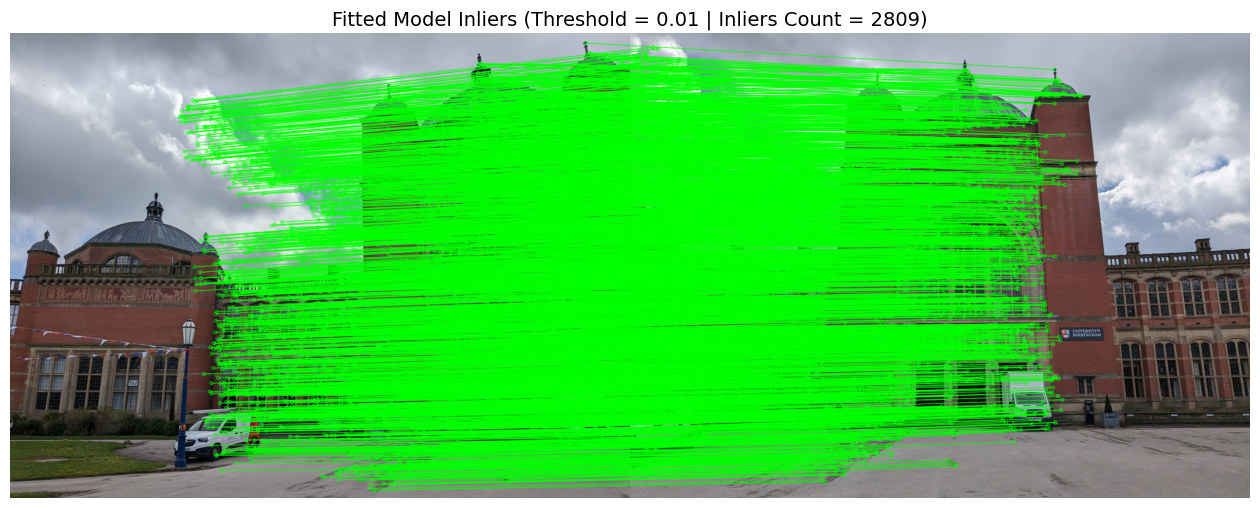
\includegraphics[width=\linewidth, height=4cm, keepaspectratio]{
                ransac_001.png
            }
            \caption{Threshold 0.01 (2809 Inliers): Hyper-sensitive threshold introducing
            high outlier ratio and noise.}
            \label{fig:match_001}
        \end{minipage}
        \hfill
        % 中图：0.05 阈值
        \begin{minipage}{0.32\textwidth}
            \centering
            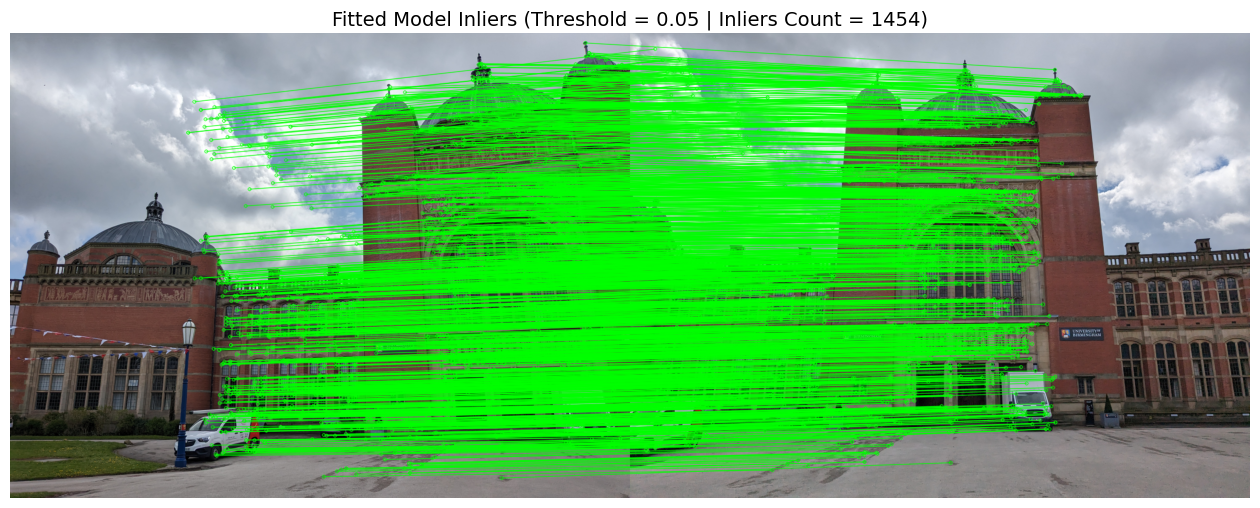
\includegraphics[width=\linewidth, height=4cm, keepaspectratio]{
                ransac_005.png
            }
            \caption{Threshold 0.05 (1454 Inliers): The optimal "sweet spot" balancing
            distinctive corners and spatial diversity.}
            \label{fig:match_005}
        \end{minipage}
        \hfill
        % 右图：0.15 阈值
        \begin{minipage}{0.32\textwidth}
            \centering
            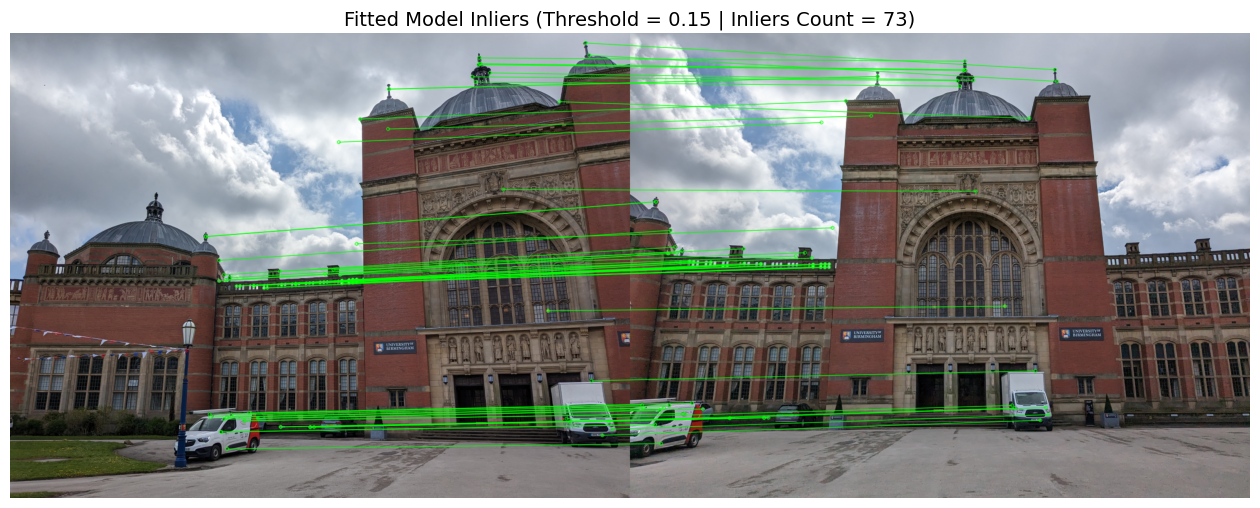
\includegraphics[width=\linewidth, height=4cm, keepaspectratio]{
                ransac_015.png
            }
            \caption{Threshold 0.15 (73 Inliers): Features are overly localized,
            increasing the risk of geometric degeneration.}
            \label{fig:match_015}
        \end{minipage}
    \end{figure*}

    \subsection{Evaluation: Robustness and Accuracy Analysis}
    Based on the quantitative data and visual evidence, I derived the following
    critical insights regarding the interplay between SIFT thresholds and RANSAC
    performance:

    \textbf{1. The Illusion of Robustness at Low Thresholds (e.g., 0.01):} Initially,
    a threshold of 0.01 yielded the highest number of inliers (2809). However,
    this does not equate to maximum robustness. A hyper-sensitive SIFT extractor
    flooded the matcher with over 10,000 weak features, capturing noise from
    flat surfaces. This massively increased the outlier ratio. In a fixed 1000-iteration
    RANSAC, a high outlier ratio significantly reduces the mathematical probability
    of sampling a pure, noise-free 4-point subset, increasing the risk of converging
    on a suboptimal local minimum and causing massive computational overhead.

    \textbf{2. The Geometric Risk of High Thresholds (e.g., 0.15):} Conversely, raising
    the threshold to 0.15 aggressively filtered out noise, leaving only 73
    highly distinct corners. While this dramatically accelerated the RANSAC computation
    and virtually eliminated false matches, it introduced a severe geometric
    risk: \textit{lack of spatial distribution}. As seen in Figure \ref{fig:match_015},
    the surviving points are heavily localized. A homography matrix derived from
    highly localized points acts as a degenerate constraint, leading to
    catastrophic stretching when extrapolated to the rest of the image.

    \textbf{3. Conclusion (The Sweet Spot):} Therefore, optimizing RANSAC is not
    merely about maximizing inliers, but balancing the \textit{outlier ratio}
    with \textit{spatial constraint diversity}. A threshold between 0.03 and
    0.05 provides the optimal "sweet spot"—it filters out flat-region noise to maintain
    a healthy inlier probability while retaining enough widely distributed strong
    corners to anchor a globally accurate geometric transformation.

    % ==========================================
    % 最终综合讨论与结论部分
    % ==========================================
    \section{Results}
    Across the three tasks, my implementations successfully recovered robust
    mathematical structures from raw image pairs. For the UOB dataset (Task 1),
    applying cylindrical projection and distance-transform blending reduced the
    RMSE from 2.599 to 2.413 pixels, yielding a distortion-free panorama. For
    the Door dataset (Task 2), implementing MAGSAC and hard-cut blending averted
    memory overflow from degenerate matrices and eliminated ghosting, bringing
    the RMSE down to 0.928 pixels on the dominant plane. Finally, the custom
    RANSAC implementation (Task 3) quantitatively demonstrated that manipulating
    the SIFT contrast threshold controls a critical trade-off between inlier
    abundance and spatial geometric diversity.
    % ==========================================
    % 最终综合讨论与结论部分 (高级学术结构)
    % ==========================================
    \section{Discussion}

    \subsection{Analysis}
    In analyzing the outcomes of the three tasks, several fundamental principles
    and limitations of computer vision pipelines were highlighted.

    \textbf{1. The Geometric Limits of 2D Homography:} The stark contrast
    between the successful UOB panorama (Task 1) and the fractured floor lines
    in the Door dataset (Task 2) reveals a critical geometric limitation. A $3 \times
    3$ homography matrix strictly assumes either a purely rotating camera around
    its optical center or a perfectly planar 3D scene. When severe translational
    parallax is introduced in close-up indoor environments, no linear 2D transformation
    can perfectly align objects at varying depths. The algorithm can effectively
    optimize for the dominant plane (the door), but residual structural fracture
    in non-coplanar regions (the wall edges) is mathematically inevitable.

    \textbf{2. Feature Quantity vs. Model Robustness in RANSAC:} My threshold
    analysis in Task 3 disproves the intuitive assumption that "more matches equal
    better alignments." A hyper-sensitive SIFT threshold (0.01) introduced catastrophic
    outlier ratios that severely degraded RANSAC's sampling probability, leading
    to memory overflow. Conversely, an overly strict threshold (0.15) caused
    features to cluster locally, generating degenerate models that failed to extrapolate
    across the entire image. Robust estimation is therefore strictly dependent
    on finding the "sweet spot" (e.g., 0.05) that balances feature
    distinctiveness with global spatial distribution.

    \subsection{Validation}
    The experimental data and visual artifacts serve to validate my context-specific
    design choices throughout the assignment.

    \textbf{1. Validation of Context-Aware Blending:} The failure of global alpha
    blending in Task 2 proves that blending strategies cannot be universally applied.
    Smooth feathering is only valid when the underlying geometry is perfectly
    aligned. In the presence of unavoidable 3D parallax, forcing a smooth blend
    created severe ghosting artifacts. Thus, switching to a hard-cut seam with
    localized feathering was a validated design choice to preserve structural
    sharpness while masking the illumination differences.

    \textbf{2. Validation through Quantitative Metrics:} The reduction of the Root
    Mean Square Error (RMSE) across the tasks explicitly validates my mathematical
    preprocessing steps. For instance, applying cylindrical projection in Task 1
    reduced the RMSE from 2.599 to 2.413 pixels, mathematically validating the
    removal of perspective stretching. Similarly, employing the MAGSAC estimator
    in Task 2 successfully bounded the reprojection error of the dominant plane
    to 0.928 pixels, validating its superiority over standard RANSAC in filtering
    degenerate, highly collinear configurations.

    % ==========================================
    % 全文总结
    % ==========================================
    \section{Conclusion}
    This assignment demonstrated that effective image stitching requires a deep
    synergy between mathematical models and physical scene constraints. Simply chaining
    black-box algorithms leads to perspective distortion, ghosting artifacts, and
    kernel crashes. By critically adapting the preprocessing geometry (cylindrical
    mapping), upgrading the robust estimators (MAGSAC), and dynamically tuning
    feature extraction thresholds to prevent RANSAC degeneration, I constructed a
    computer vision pipeline that is both computationally robust and visually accurate.

    % ==========================================
    % 致谢部分 (选填，显得有礼貌且专业)
    % ==========================================
    \section*{ACKNOWLEDGEMENTS}
    I would like to thank the teaching team of the Robotic Vision module at the University
    of Birmingham for providing the diverse datasets (UOB and Door) and the foundational
    lecture materials that guided the design choices in this assignment.

    % ==========================================
    % 参考文献 (放入我们这次用到的核心算法的原始论文)
    % ==========================================
    % ==========================================
    % 参考文献 (标准 LaTeX 格式)
    % ==========================================
    \begin{thebibliography}{99}
        \bibitem{lowe2004} Lowe, D. G. (2004). Distinctive image features from scale-invariant
            keypoints. \textit{International journal of computer vision}, 60(2),
            91-110.

        \bibitem{fischler1981} Fischler, M. A., \& Bolles, R. C. (1981). Random sample
            consensus: a paradigm for model fitting with applications to image
            analysis and automated cartography. \textit{Communications of the
            ACM}, 24(6), 381-395.

        \bibitem{bradski2000} Bradski, G. (2000). The OpenCV Library. \textit{Dr.
            Dobb's Journal of Software Tools}.
    \end{thebibliography}
\end{document}